\documentclass{article}
\usepackage[utf8]{inputenc}
%% Sets page size and margins
\usepackage[a4paper,top=2cm,bottom=2cm,left=2cm,right=2cm,marginparwidth=1.75cm]{geometry}

\usepackage{algorithm}
\usepackage{algorithmic}
\usepackage{float}
\renewcommand{\algorithmicrequire}{ \textbf{Input:}} %Use Input in the format of Algorithm
\renewcommand{\algorithmicensure}{ \textbf{Output:}} %UseOutput in the format of Algorithm
\usepackage{multirow}
%\usepackage{fdsymbol}
\usepackage{amsthm}
%% Useful packages
\usepackage{amsmath}
\usepackage{amssymb}
\usepackage{latexsym}
%\usepackage{fdsymbol} 
\usepackage{ dsfont }
\usepackage{color}
\usepackage{bm}
\usepackage{graphicx}
\usepackage[export]{adjustbox}
\usepackage[colorinlistoftodos]{todonotes}
\usepackage[colorlinks=true, allcolors=blue]{hyperref}
\usepackage{biblatex}
\addbibresource{references.bib}

\title{Plots of Subgradient}
%\author{Wei Kuang}
%\date{June 29, 2023}

\begin{document}

\maketitle
\section{ADMM}
The objective function is
\begin{equation}
    f(\beta) = \frac{1}{2}\|z-M_{\perp}\beta\|^2 + \lambda\|\beta\|_1,
\end{equation}
thus the subgradient we care about is
\begin{equation}
    \partial f(\beta) = M_{\perp}^T(M_{\perp}\beta-z) + \lambda \partial \|\beta\|_1.
\end{equation}

\begin{figure}[H]
	\centering
	\subfigure{
		\begin{minipage}[b]{1\textwidth}
			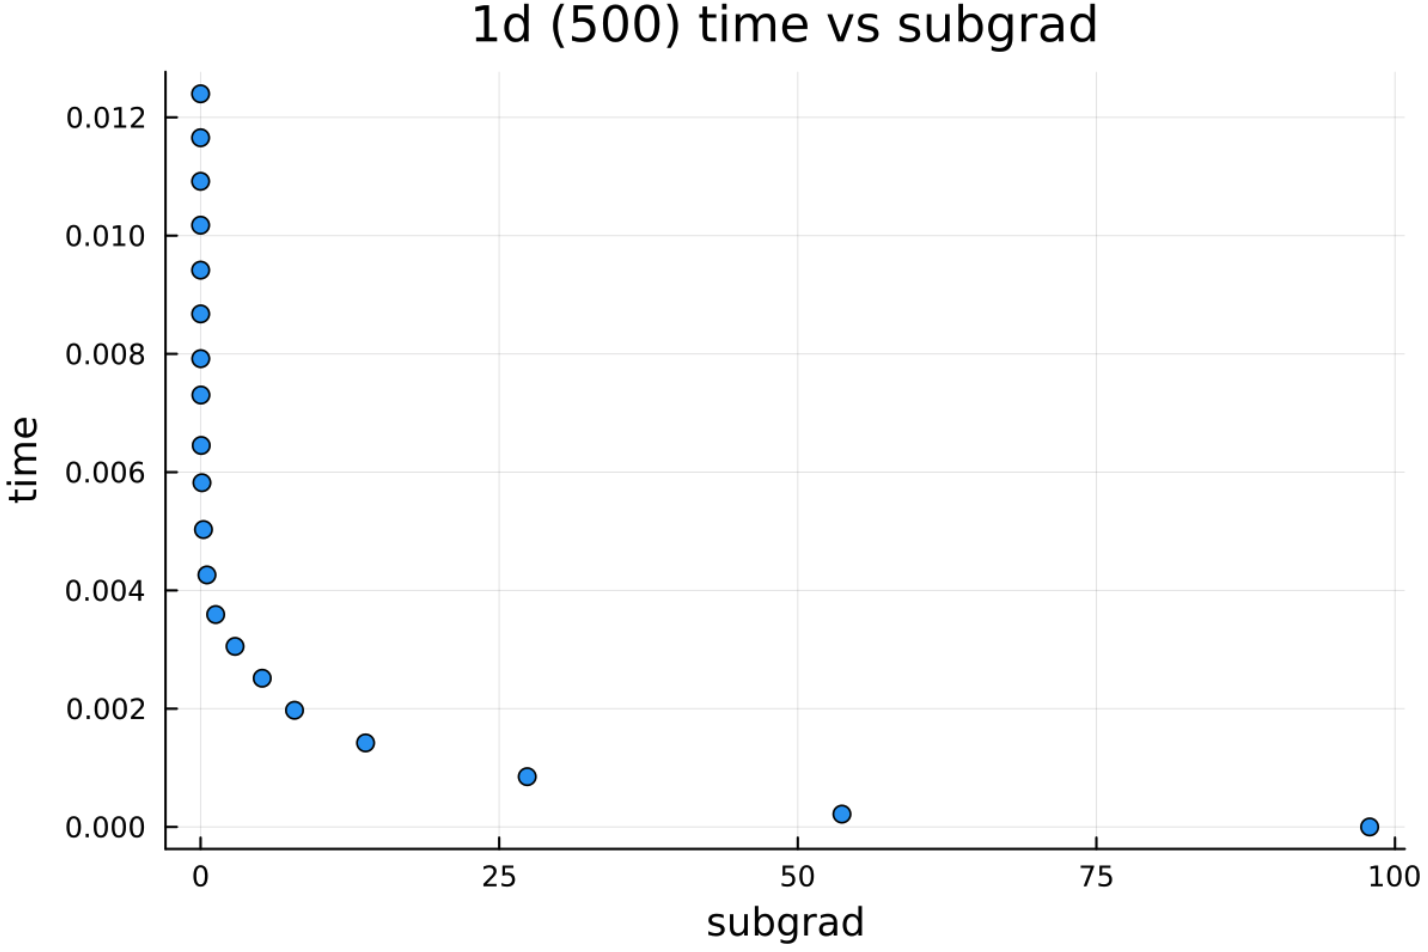
\includegraphics[width=0.3\textwidth]{Interior Point Method/subgradplot2_fig/1dtimevssubgrad.png} 			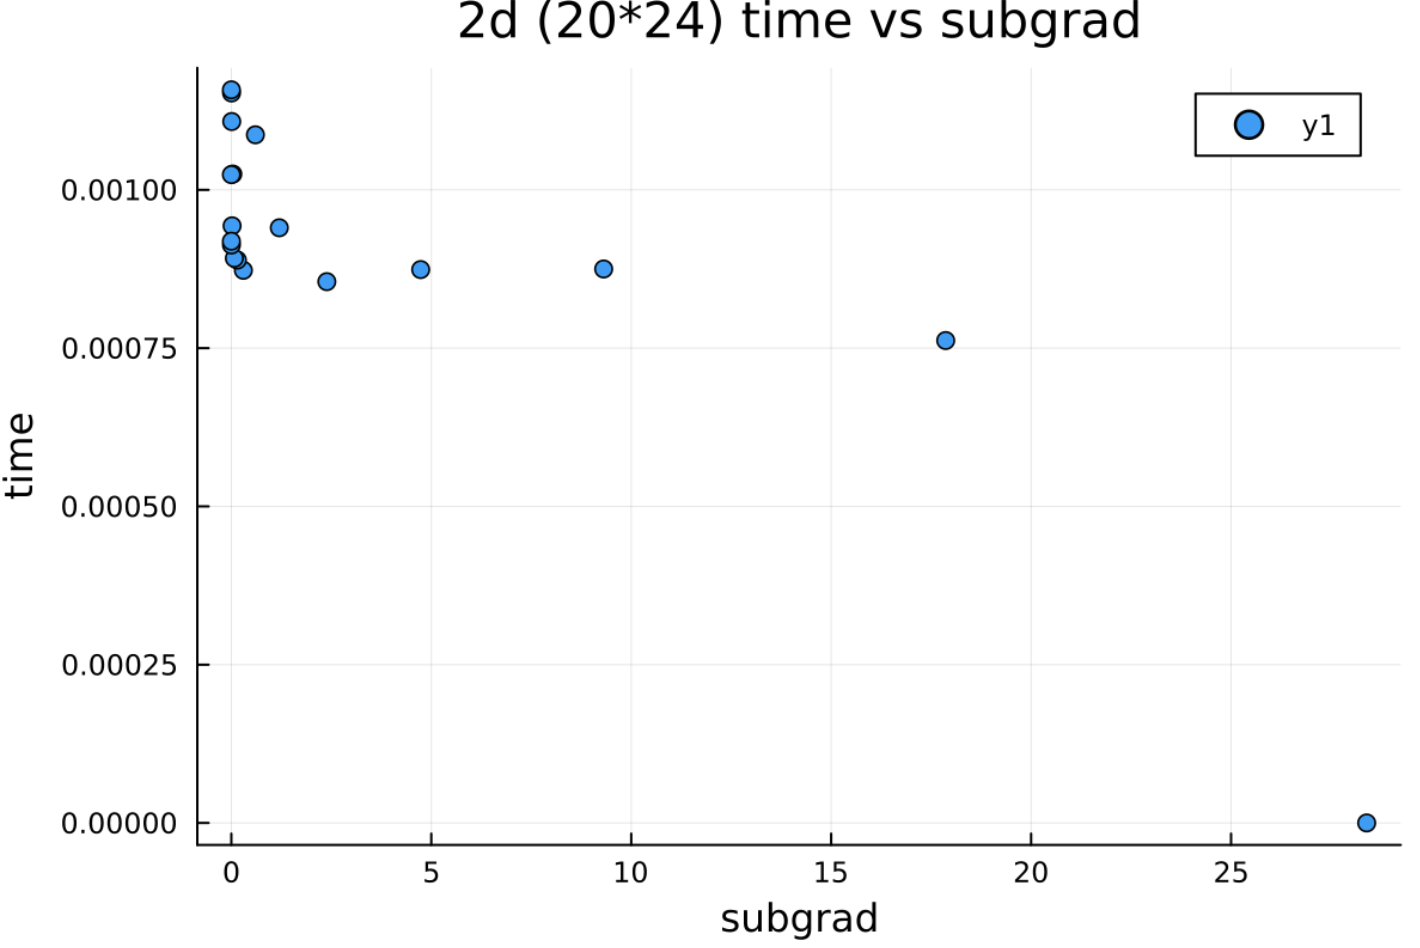
\includegraphics[width=0.3\textwidth]{Interior Point Method/subgradplot2_fig/2dtimevssubgrad.png}
          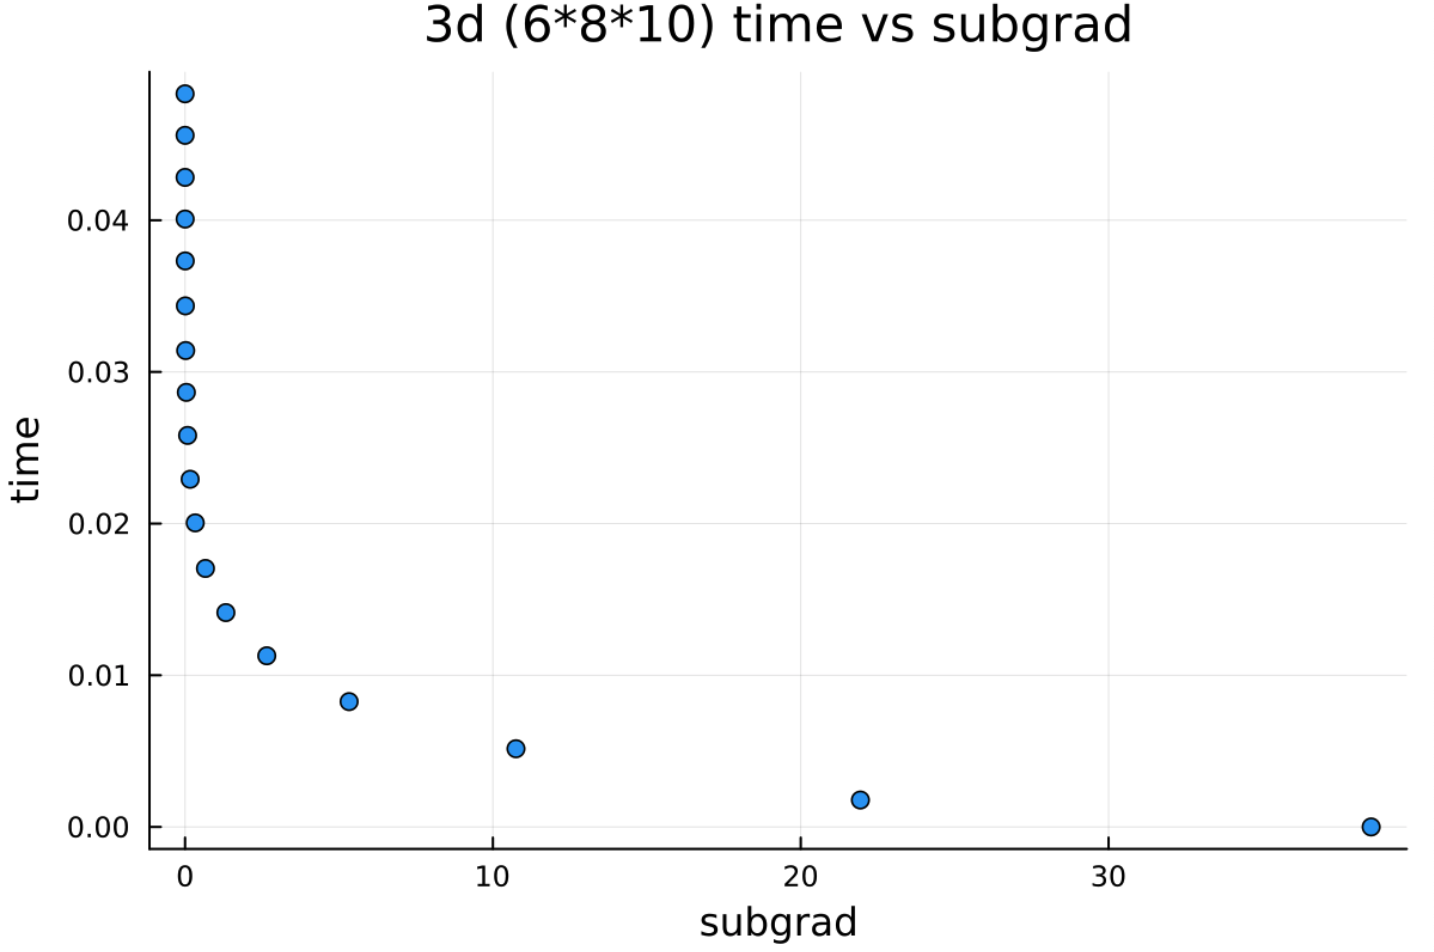
\includegraphics[width=0.3\textwidth]{Interior Point Method/subgradplot2_fig/3dtimevssubgrad.png}
		\end{minipage}
  \caption{ADMM: cumulated time vs subgrad}
	}
    	\subfigure{
    		\begin{minipage}[b]{1\textwidth}
   		 	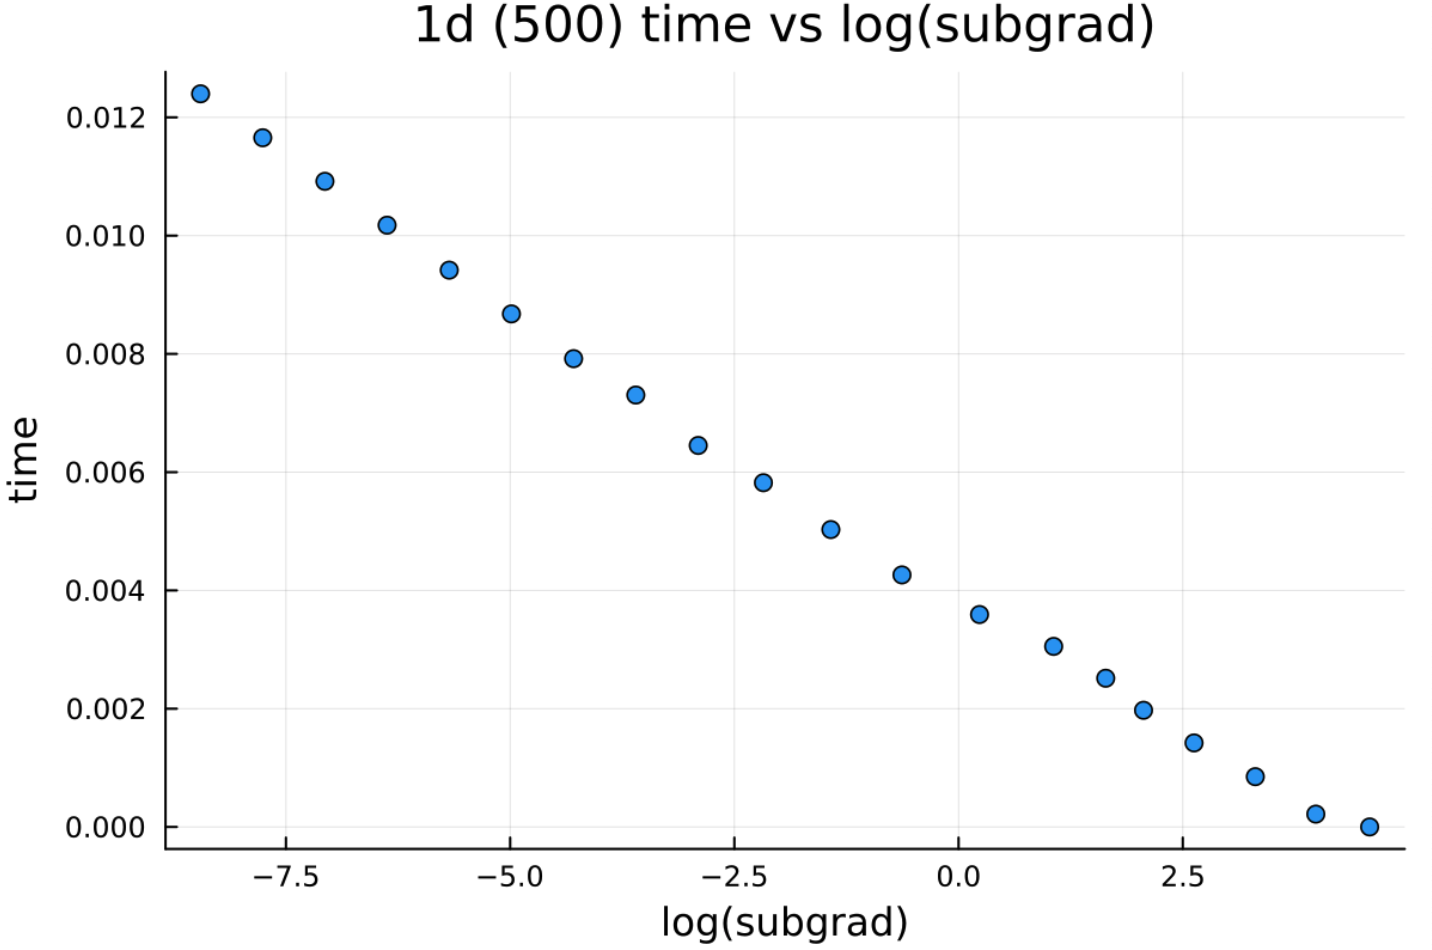
\includegraphics[width=0.3\textwidth]{Interior Point Method/subgradplot2_fig/1dtimevslogsubgrad.png}		 	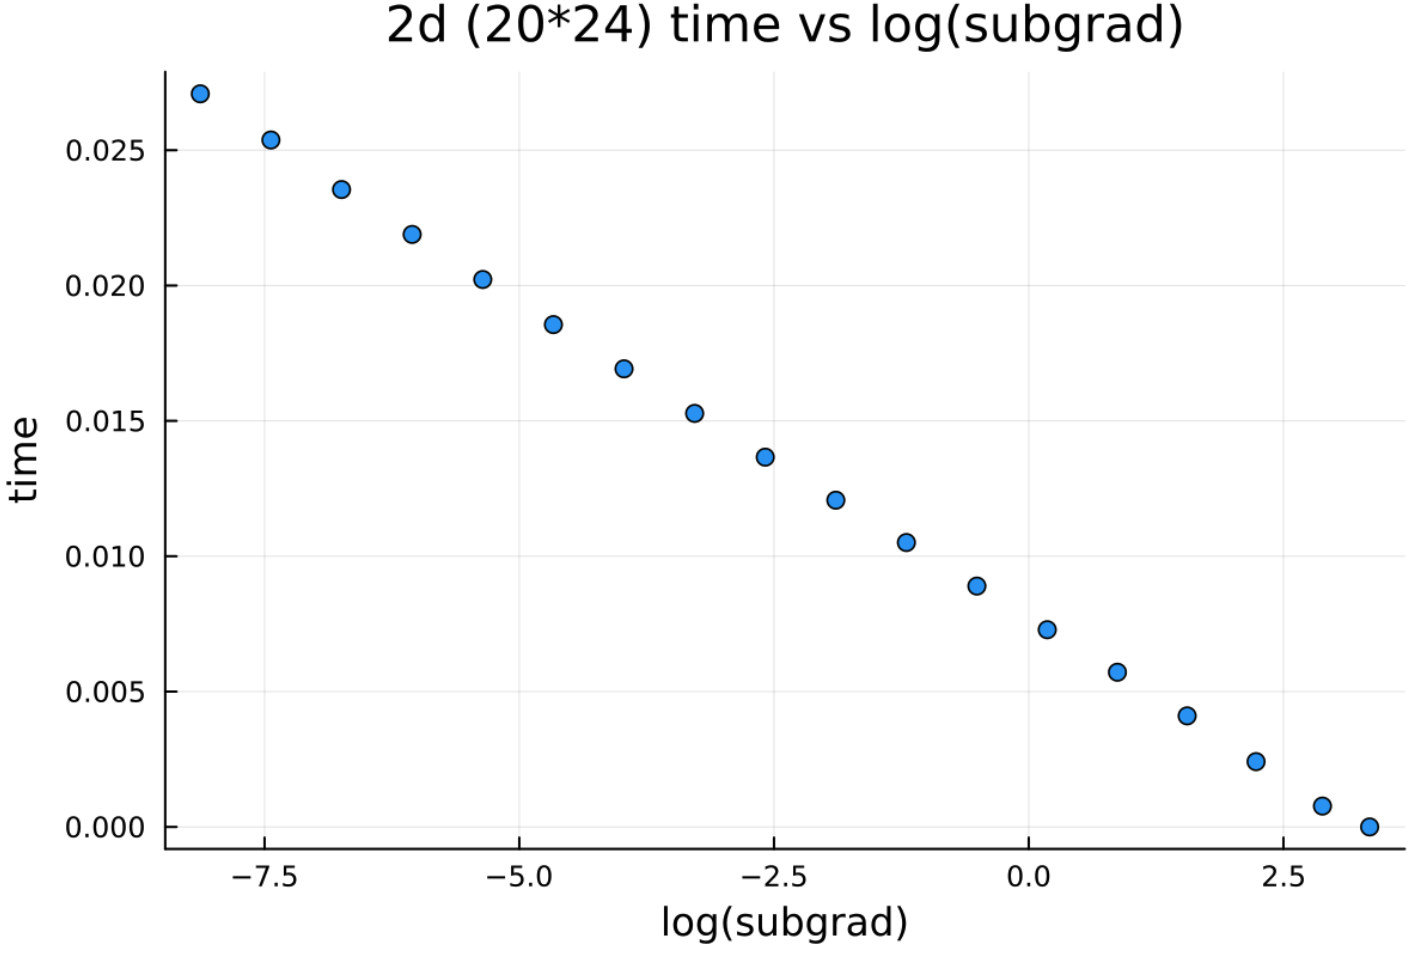
\includegraphics[width=0.3\textwidth]{Interior Point Method/subgradplot2_fig/2dtimevslogsubgrad.png}           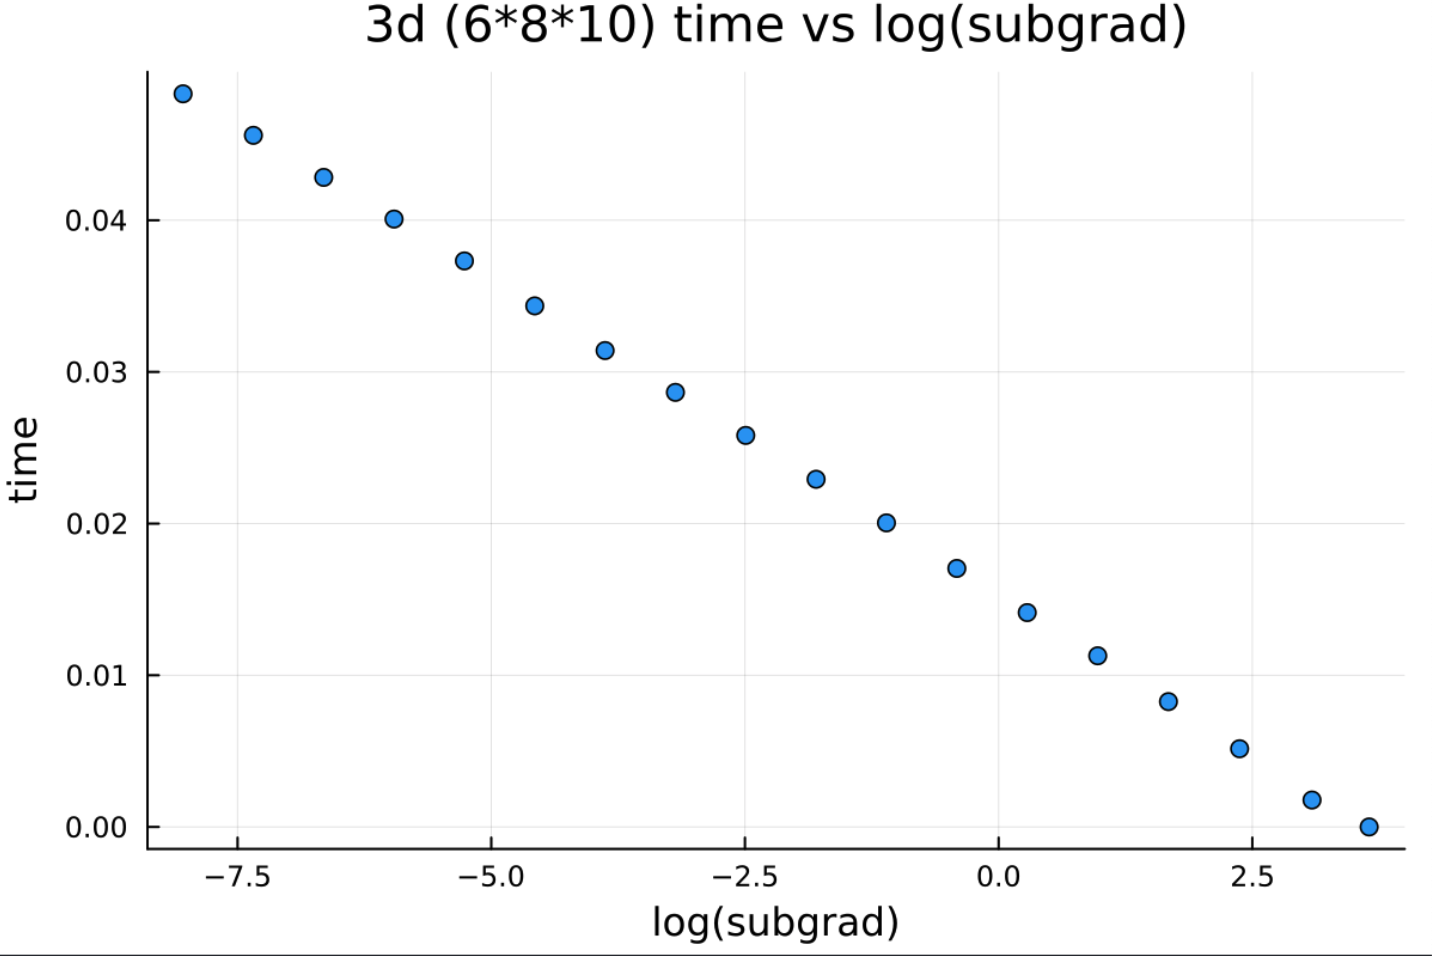
\includegraphics[width=0.3\textwidth]{Interior Point Method/subgradplot2_fig/3dtimevslogsubgrad.png}
    		\end{minipage}
      \caption{ADMM: cumulated time vs log(subgrad)}
		}
   	\subfigure{
    		\begin{minipage}[b]{1\textwidth}
   		 	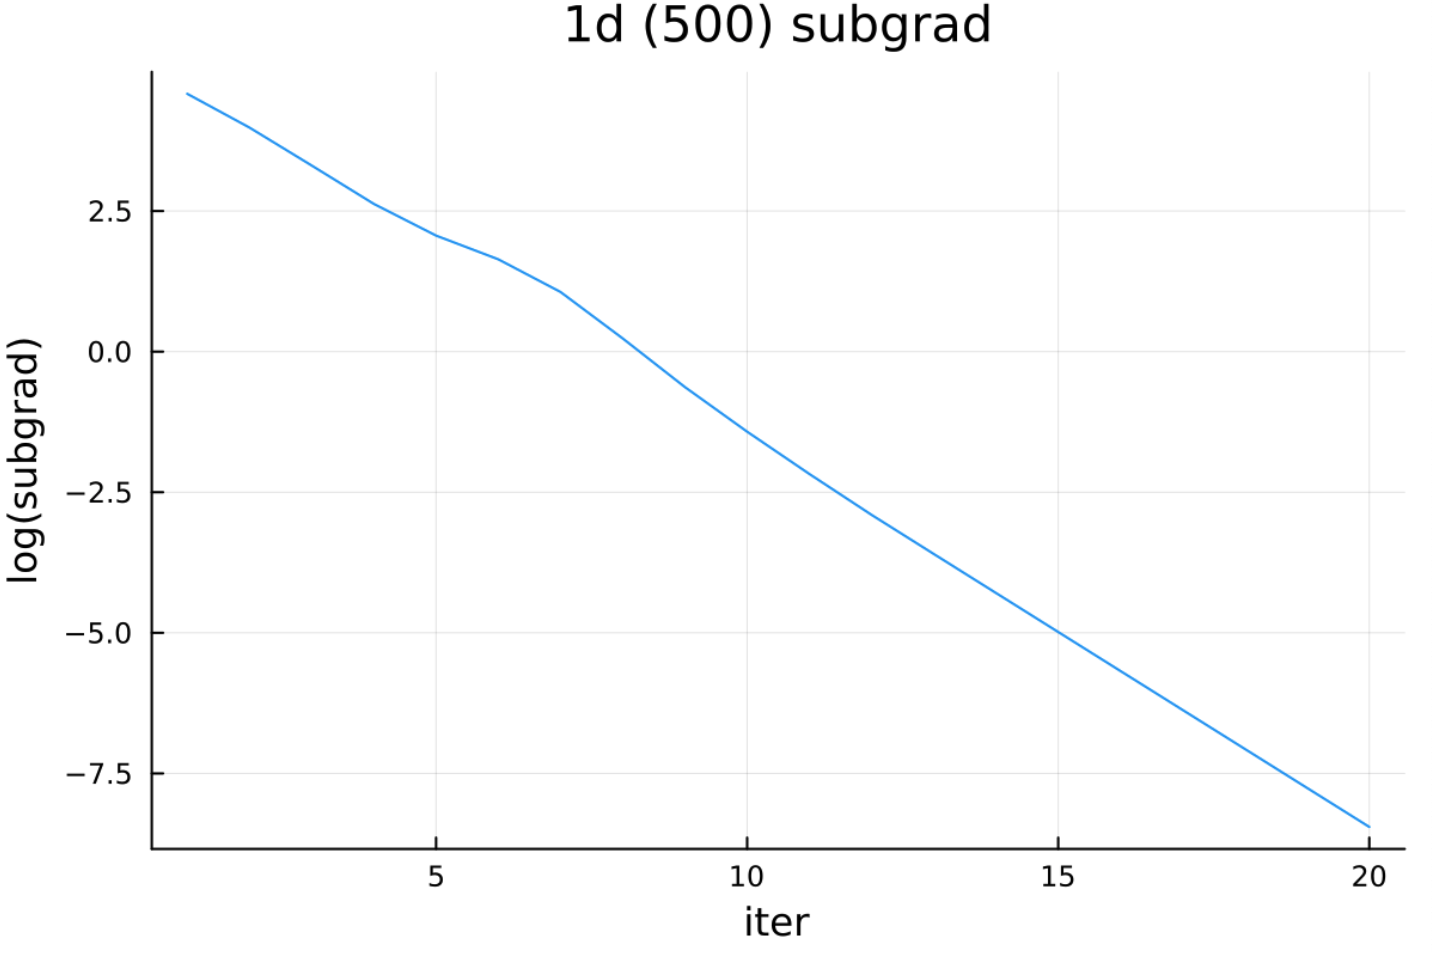
\includegraphics[width=0.3\textwidth]{Interior Point Method/subgradplot2_fig/1dlogsubgrad.png}		 	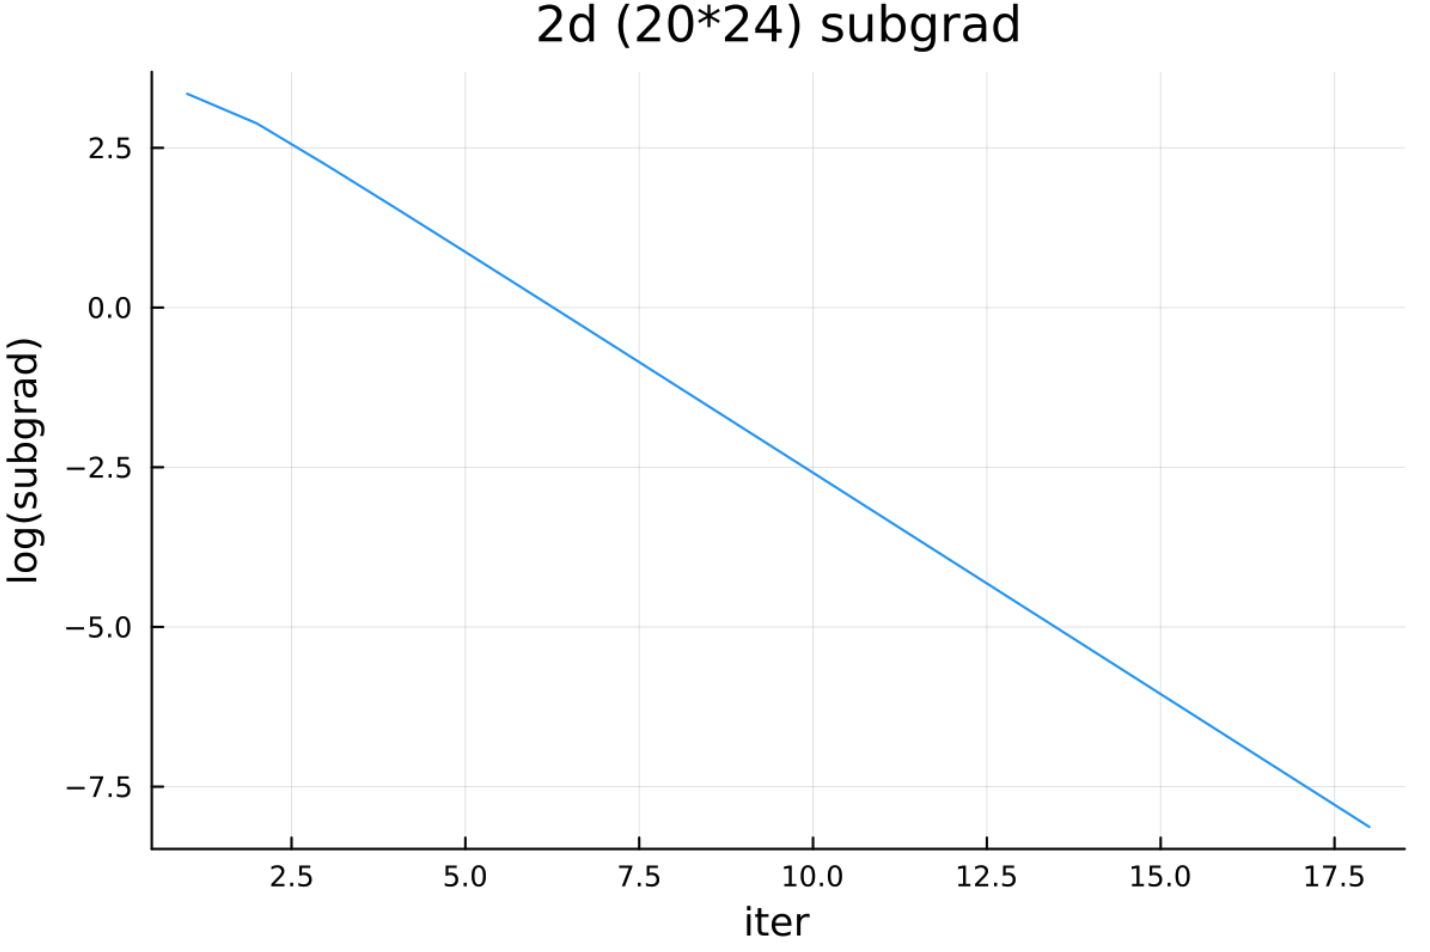
\includegraphics[width=0.3\textwidth]{Interior Point Method/subgradplot2_fig/2dlogsubgrad.png}           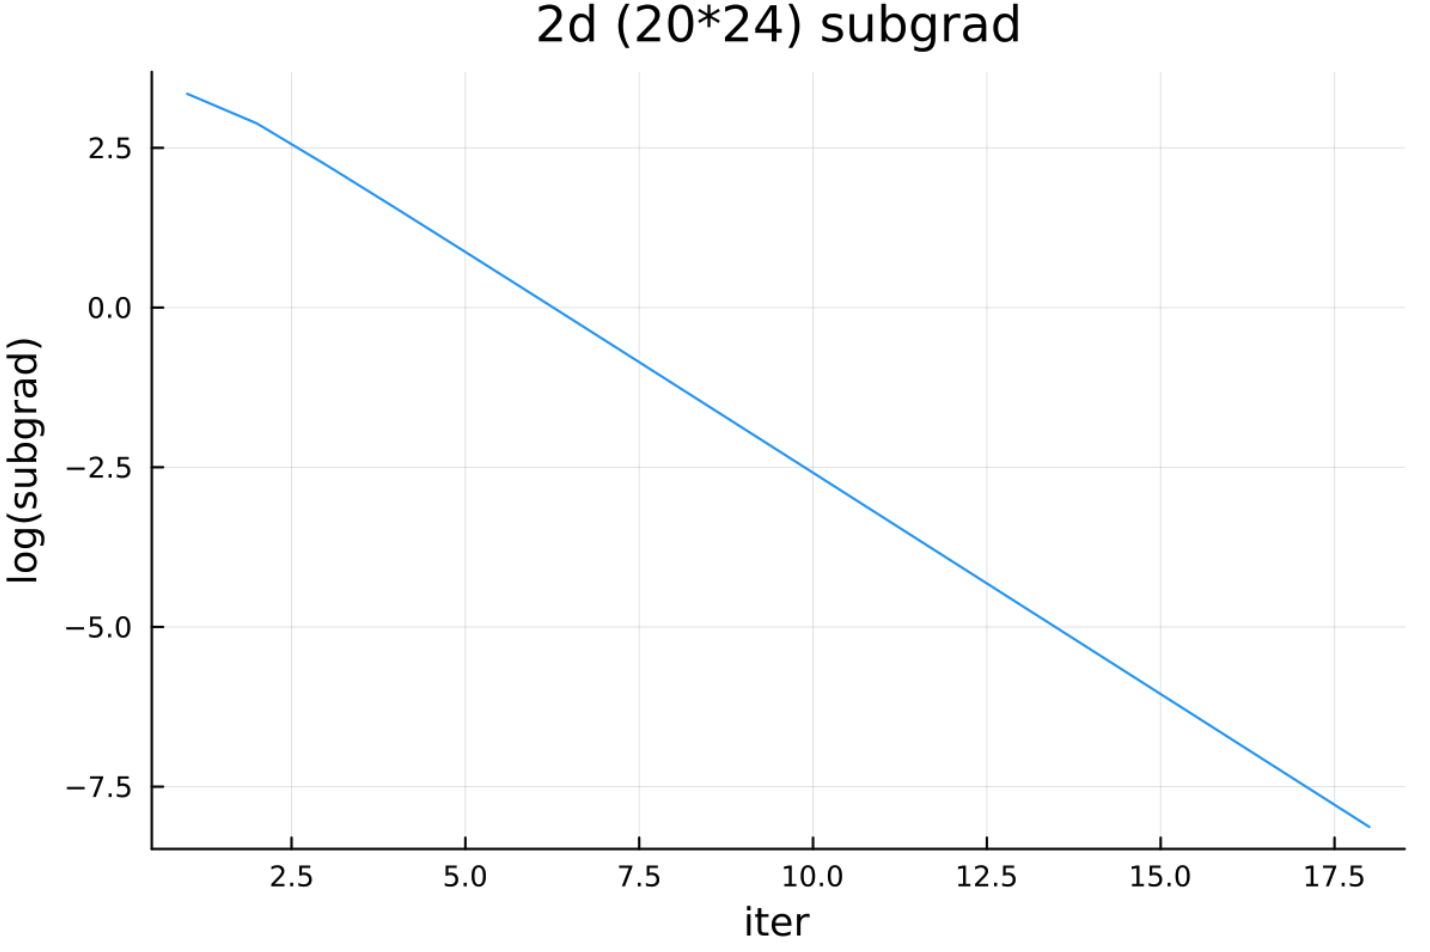
\includegraphics[width=0.3\textwidth]{Interior Point Method/subgradplot2_fig/2dlogsubgrad.png}
    		\end{minipage}
      \caption{ADMM: log(subgrad) vs iter}
		}  
\end{figure}

\section{Primal IPOPT}
We start with the problem
\begin{equation}
    \min_{\beta} \frac{1}{2}\|z-M_{\perp}\beta\|^2 \text{ s.t }\|\beta\|_1\leq d.
\end{equation}
To make the constraint differentiable, we rewrite the problem as
\begin{equation}
    \begin{aligned}
        \min_{\beta} &\frac{1}{2}\|z-M_{\perp}\beta\|^2\\
        \text{s.t. }&l_i = -\beta_i-c_i\leq 0\\
        &u_i = \beta_i-c_i\leq 0\\
        &g = \sum_{i}c_i-d\leq 0
    \end{aligned}
\end{equation}
The Lagrangian of the problem is
\begin{equation}
    L(\beta,c; \xi,\eta,\lambda)= 
     \frac{1}{2}\|z-M_{\perp}\beta\|^2
     +\sum_{i}\xi_i(-\beta_i-c_i)
     +\sum_{i}\eta_i(\beta_i-c_i)
     + \lambda(\sum_{i}c_i-d).
\end{equation}
If $(\beta^\star, c^\star, \xi^\star, \eta^\star, \lambda^\star)$ is a local solution, then it has to satisfies the following KKT condition:
\begin{equation}
    \begin{aligned}
        0\in &\partial_{\beta, c}L(\beta^\star, c^\star; \xi^\star, \eta^\star, \lambda^\star) = \begin{pmatrix}
            M_{\perp}^T(M_{\perp}-z)-\xi+\eta\\
            -\xi-\eta+\lambda\boldsymbol{1}
        \end{pmatrix}\\
        &\xi^\star, \eta^\star, \lambda^\star \geq 0\\
        &\xi^\star\odot (-\beta^\star-c^\star)=0\\ &\eta^\star\odot(\beta^\star-c^\star)=0\\ &\lambda^\star(\sum_{i}c_i^\star-d)=0      
    \end{aligned}
\end{equation}
We denote the penalty parameter in ADMM as $\lambda_A$ and the corresponding solution of it is $\beta^\star_A$, then let $\beta^\star = \beta^\star_A$, $c^\star = |\beta^\star|$, $\lambda^\star = \lambda_A$, $d = \|\beta_A^\star\|_1$. According to the optimality condition in ADMM, we know that
\begin{equation}
    0\in\partial f(\beta^\star_A) = M_{\perp}^T(M_{\perp}\beta-z) + \lambda_A \partial \|\beta_A^\star\|_1
\end{equation}
Since $\beta_i=c_i$ and $\beta_i=-c_i$ cannot hold at the same time, thus $\xi_i=0$ if $\beta_i=-c_i$ and $\eta_i=0$ if $\beta_i=c_i$. Collect all the indices satisfying $\beta_i=c_i$ in the set $\mathcal{I}$ and the rest in $\mathcal{I}^C$. Let $\xi^\star_{\mathcal{I}}=-\lambda_A\boldsymbol{1}$ and $\xi^\star_{\mathcal{I}^C}=\boldsymbol{0}$, and $\eta^\star_{\mathcal{I}}=\boldsymbol{0}$ and $\eta^\star_{\mathcal{I}^C}=-\lambda_A\boldsymbol{1}$ then it is easy to check that the following equations hold.
\begin{equation}
    \begin{aligned}
        \begin{pmatrix}
        -\xi^\star_\mathcal{I}\\
        \eta^\star_{\mathcal{I}^C}
        \end{pmatrix}\in \lambda_A\partial\|\beta^\star_A\|_1\\
        -\begin{pmatrix}
            \xi_{\mathcal{I}}\\
            \eta_{\mathcal{I}^C}
        \end{pmatrix} = \lambda_A\boldsymbol{1}
    \end{aligned}
\end{equation}
Therefore, $(\beta_A^\star, c^\star; \xi^\star, \eta^\star,\lambda_A)$ defined above satisfies the KKT condition.

Based on the analysis above, we define $d = \sum_{i}|\beta^\star_A|$ and perform primal IPOPT. At each iteration, we compute the subgradient
\begin{equation}
    \partial f(\beta_t) = M_{\perp}^T(M_{\perp}\beta_t-z) + \lambda_A \partial \|\beta_t\|_1.
\end{equation}
The following are the plots.
\begin{figure}[H]
	\centering
	\subfigure{
		\begin{minipage}[b]{1\textwidth}
			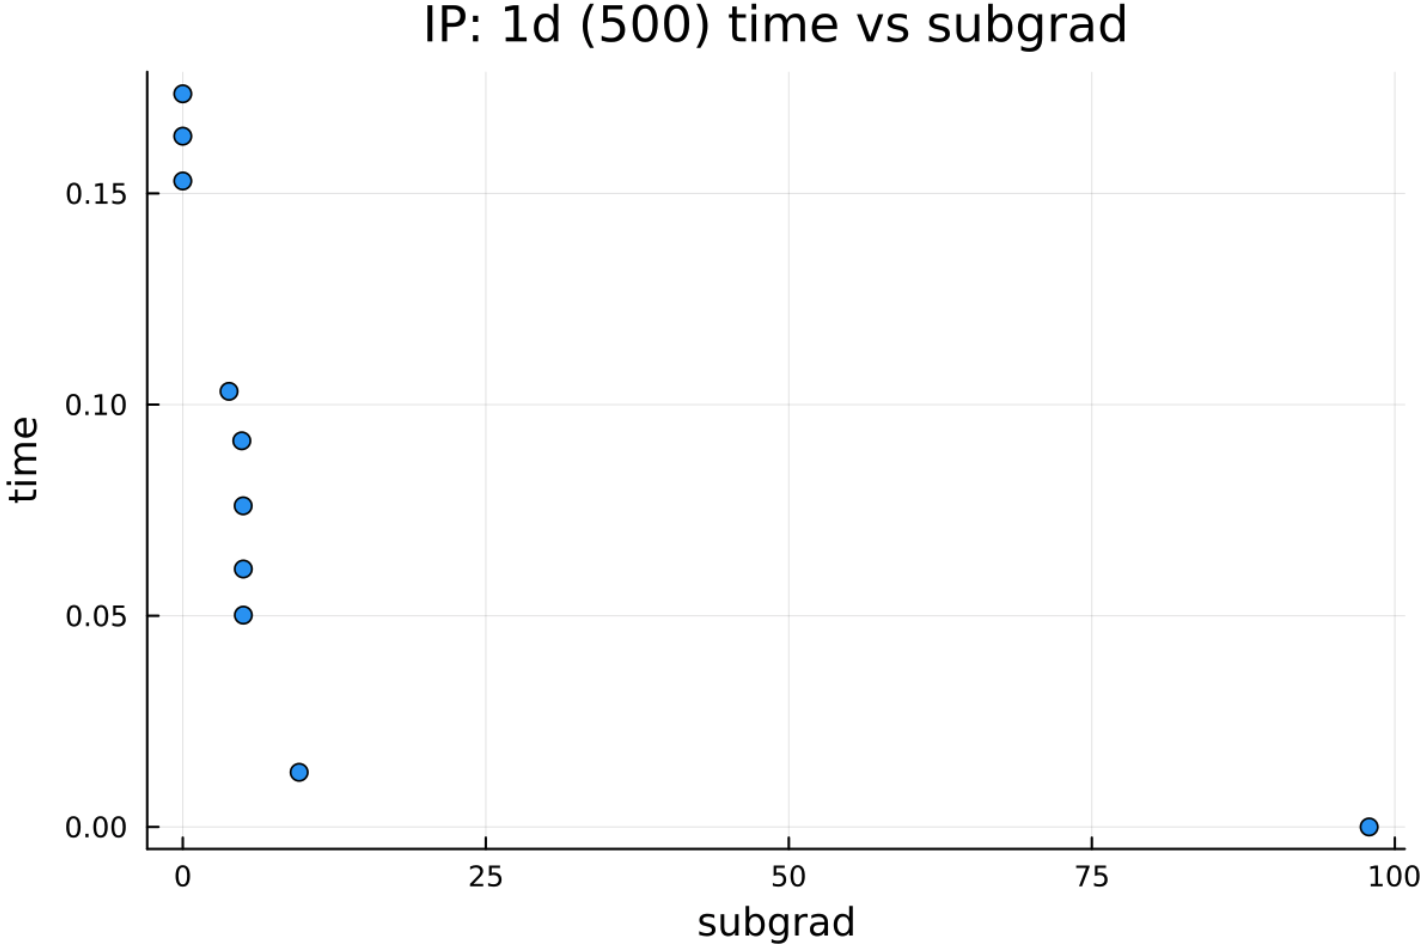
\includegraphics[width=0.3\textwidth]{Interior Point Method/subgradplot2_fig/1dIPtimevssubgrad.png} 			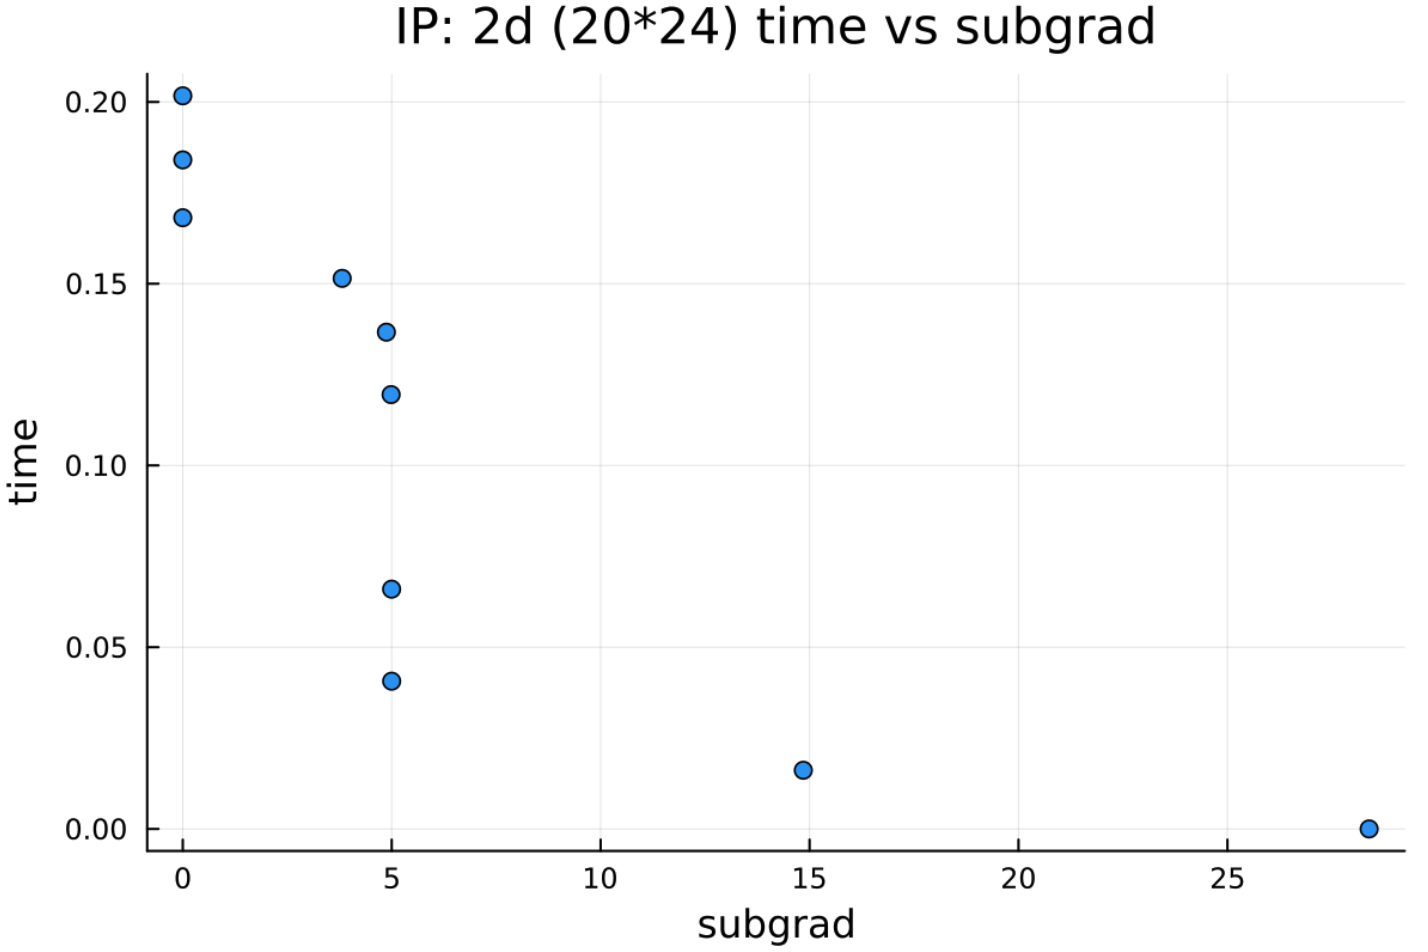
\includegraphics[width=0.3\textwidth]{Interior Point Method/subgradplot2_fig/2dIPtimevssubgrad.png}
          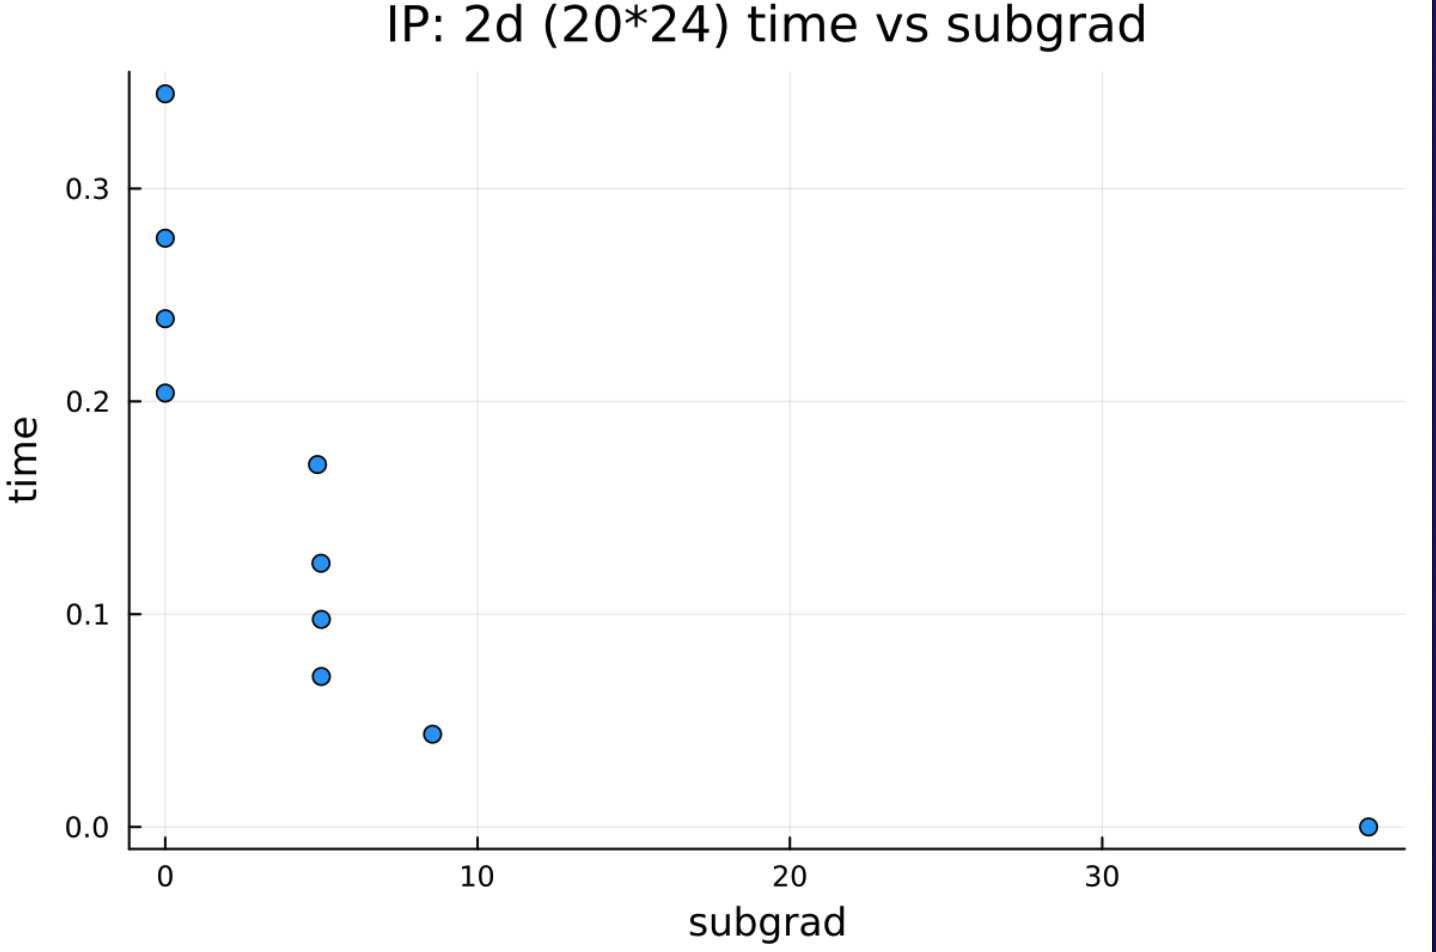
\includegraphics[width=0.3\textwidth]{Interior Point Method/subgradplot2_fig/3dIPtimevssubgrad.png}
		\end{minipage}
  \caption{IP: cumulated time vs subgrad}
	}

\end{figure}

\begin{figure}[H]
\centering
    	\subfigure{
    		\begin{minipage}[b]{1\textwidth}
   		 	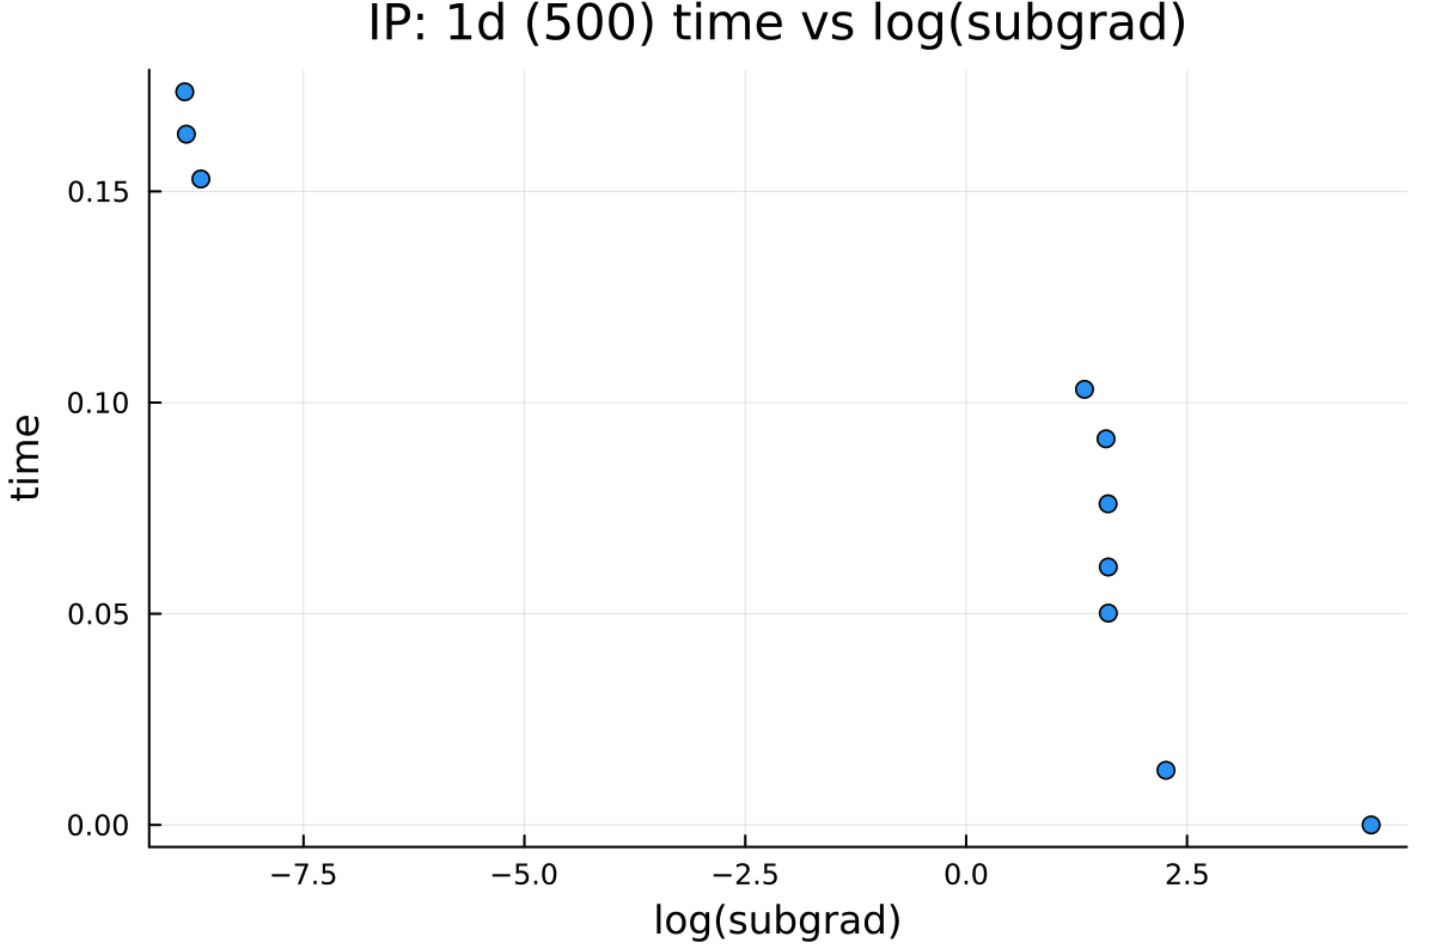
\includegraphics[width=0.3\textwidth]{Interior Point Method/subgradplot2_fig/1dIPtimevslogsubgrad.png}		 	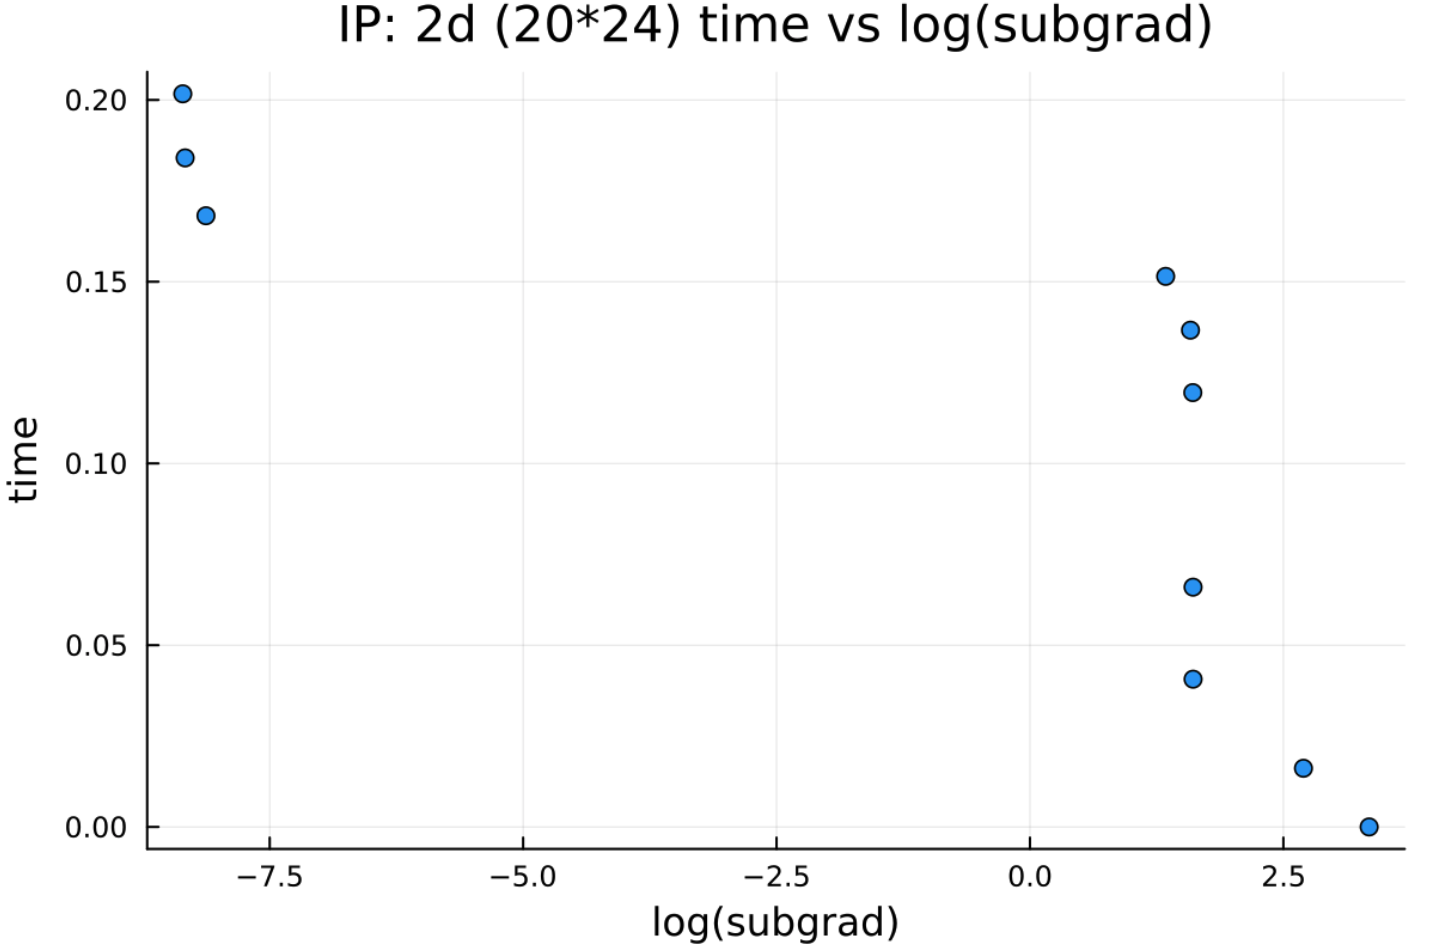
\includegraphics[width=0.3\textwidth]{Interior Point Method/subgradplot2_fig/2dIPtimevslogsubgrad.png}           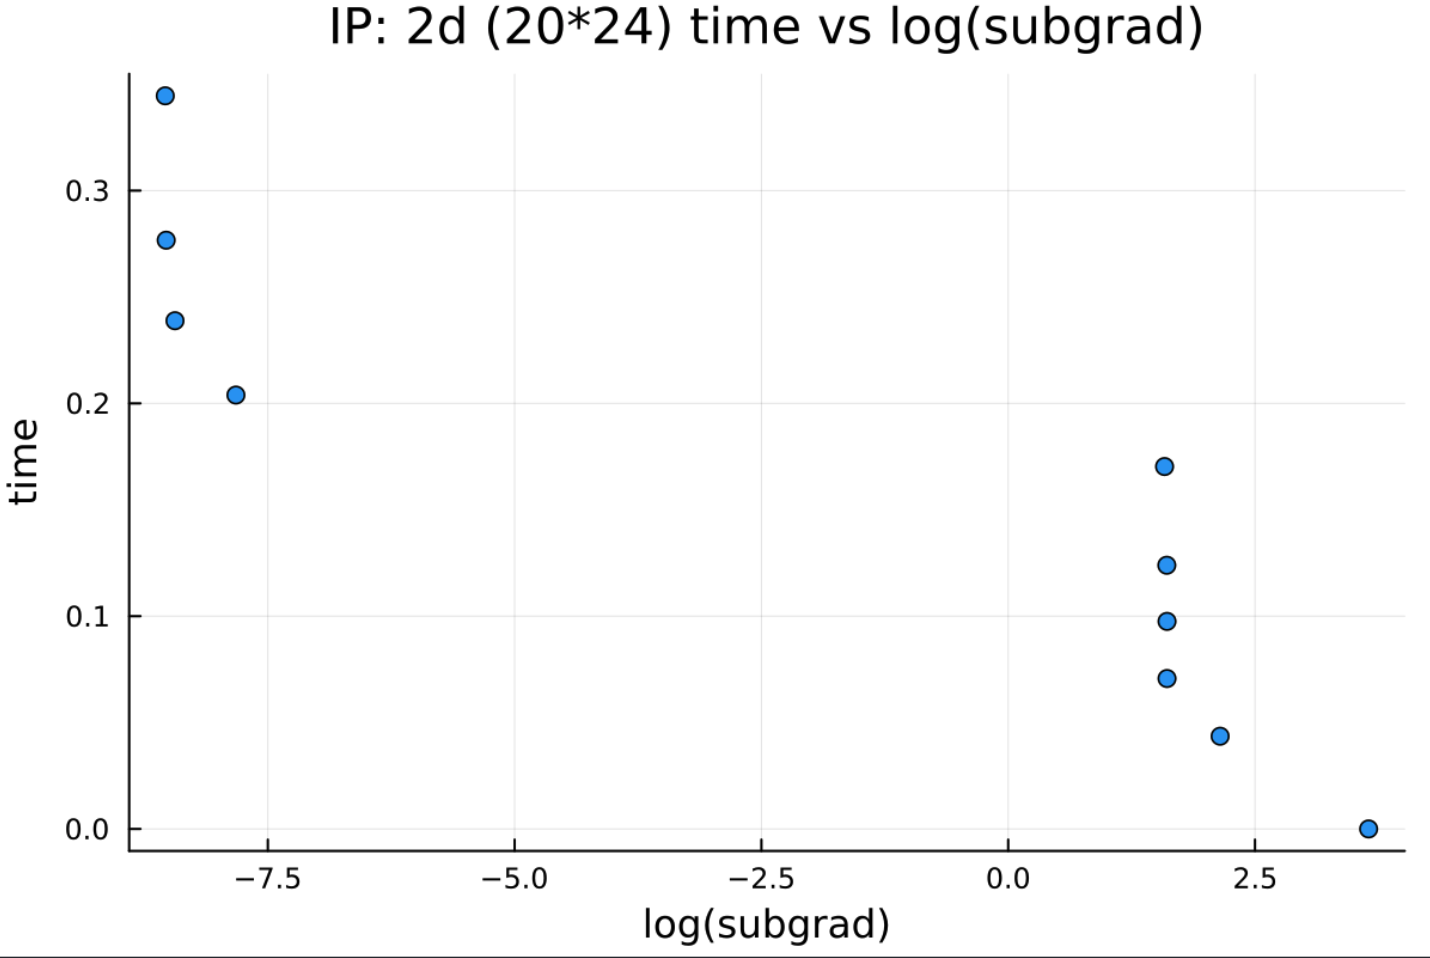
\includegraphics[width=0.3\textwidth]{Interior Point Method/subgradplot2_fig/3dIPtimevslogsubgrad.png}
    		\end{minipage}
      \caption{IP: cumulated time vs log(subgrad)}
		}
   	\subfigure{
    		\begin{minipage}[b]{1\textwidth}
   		 	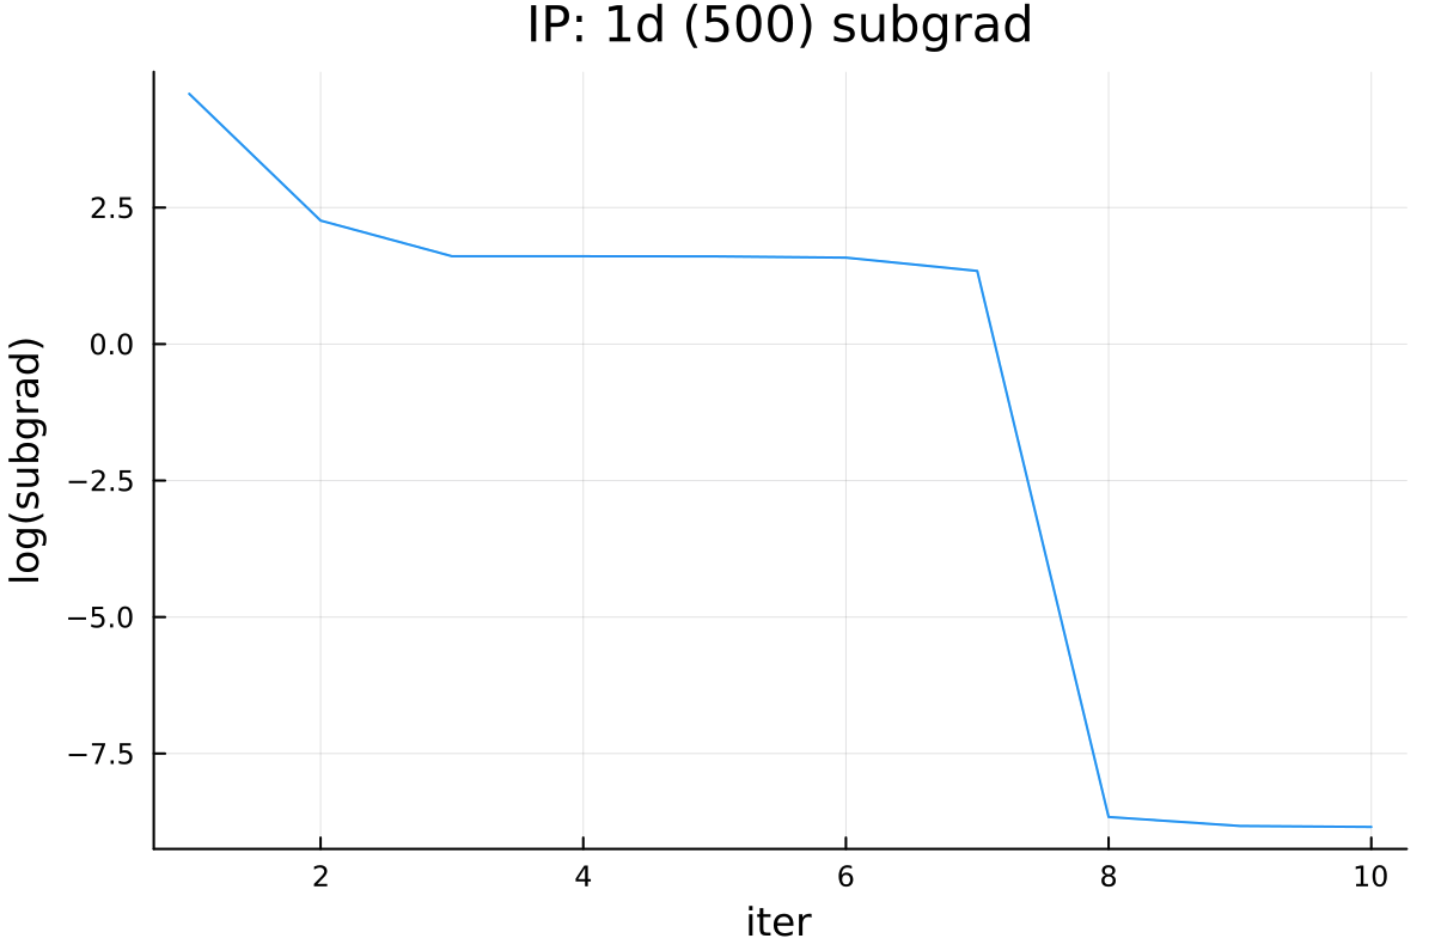
\includegraphics[width=0.3\textwidth]{Interior Point Method/subgradplot2_fig/1dIPlogsubgrad.png}		 	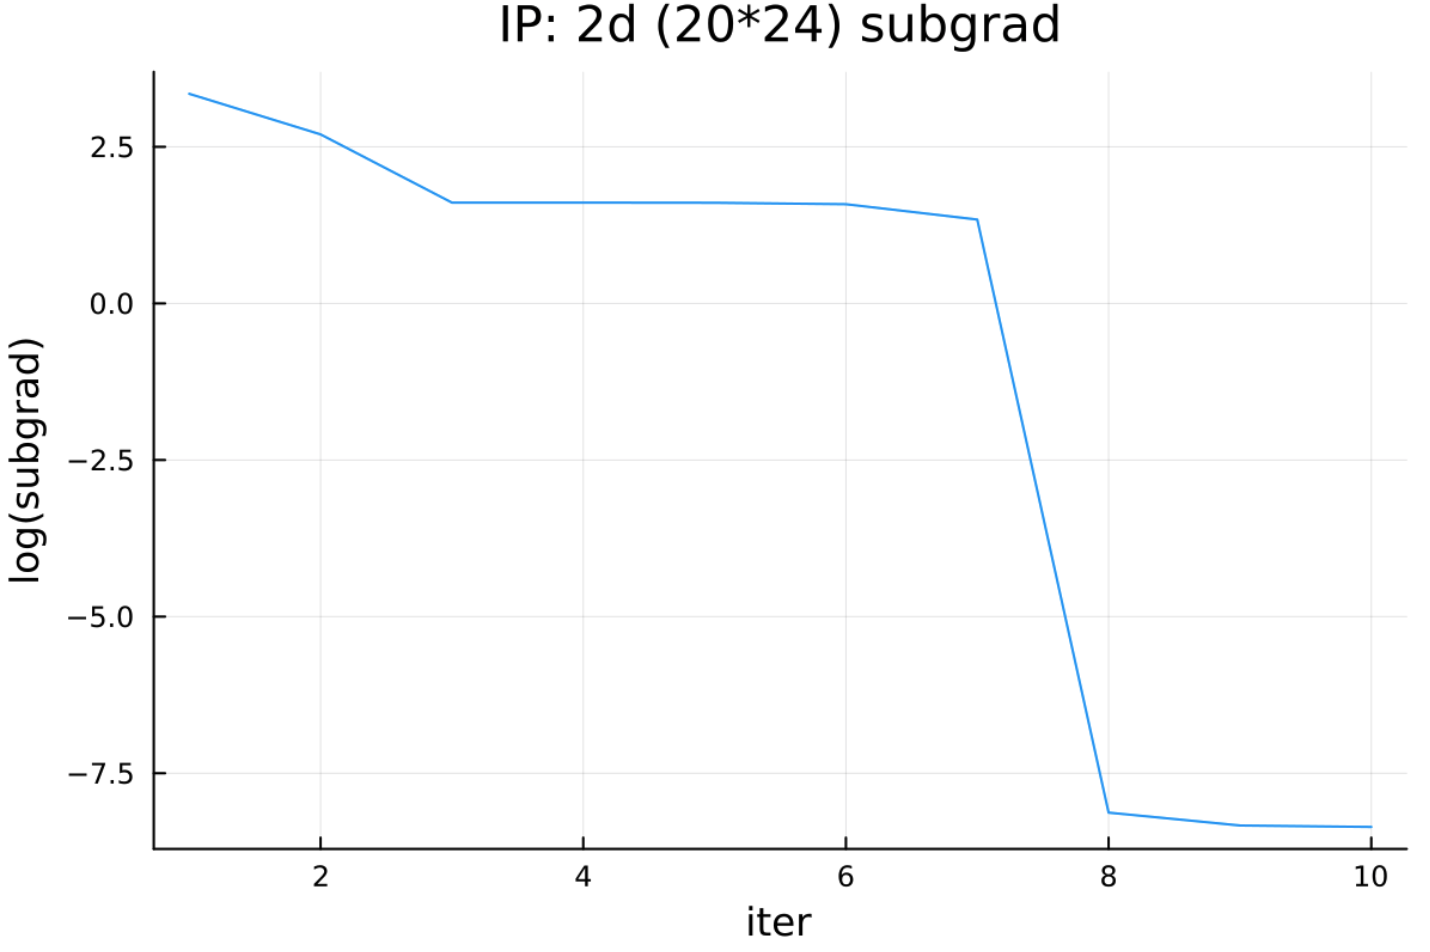
\includegraphics[width=0.3\textwidth]{Interior Point Method/subgradplot2_fig/2dIPlogsubgrad.png}           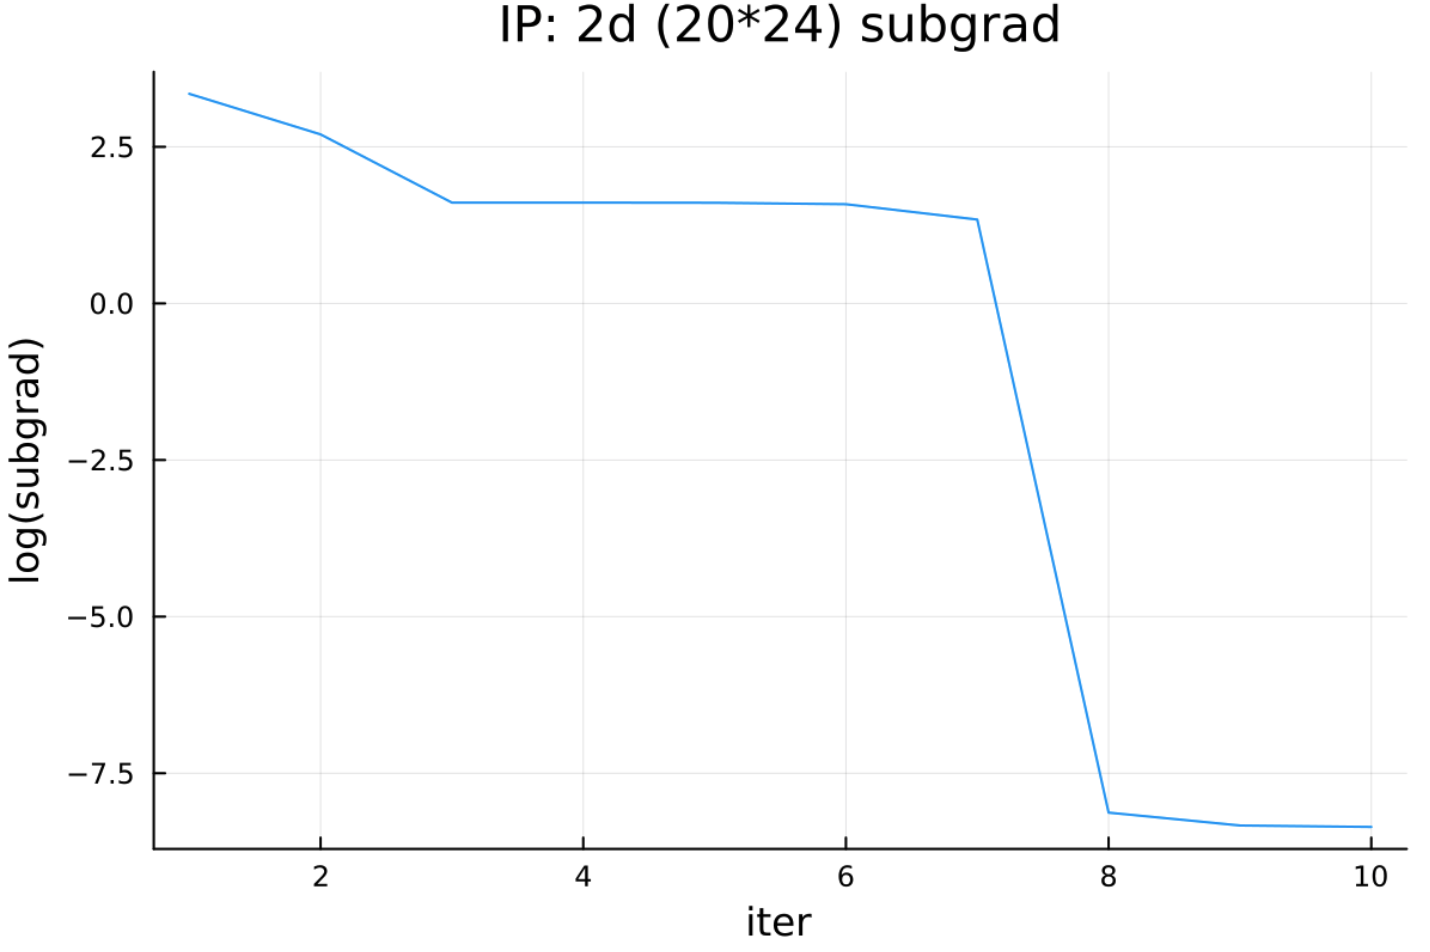
\includegraphics[width=0.3\textwidth]{Interior Point Method/subgradplot2_fig/2dIPlogsubgrad.png}
    		\end{minipage}
      \caption{IP: log(subgrad) vs iter}
		}  
\end{figure}
\section{Primal-Dual IPOPT}
The second comparison is to obtain the optimal primal-dual pair $(\beta_{PD}^\star, c_{PD}^\star, \xi_{PD}^\star, \eta_{PD}^\star, \lambda_{PD}^\star)$ of the rewritten $l_1$ constarined problem. Then we compute the following subgradient at each iteration:
\begin{equation}
    M_{\perp}^T(M_{\perp}\beta_t-z) + \lambda_{PD}^\star \partial \|\beta_t\|_1
\end{equation}

In order to obtain the primal-dual pair, we first describe the primal-dual IPOPT algorithm. If we consider the problem
\begin{equation}
    \min_x f_0(x) \text{ s.t. } f_i(x)\leq 0, i=1,\dots,m.
\end{equation}
The primal-dual IPOPT algorithm is given as
\begin{figure}[H]
	\centering	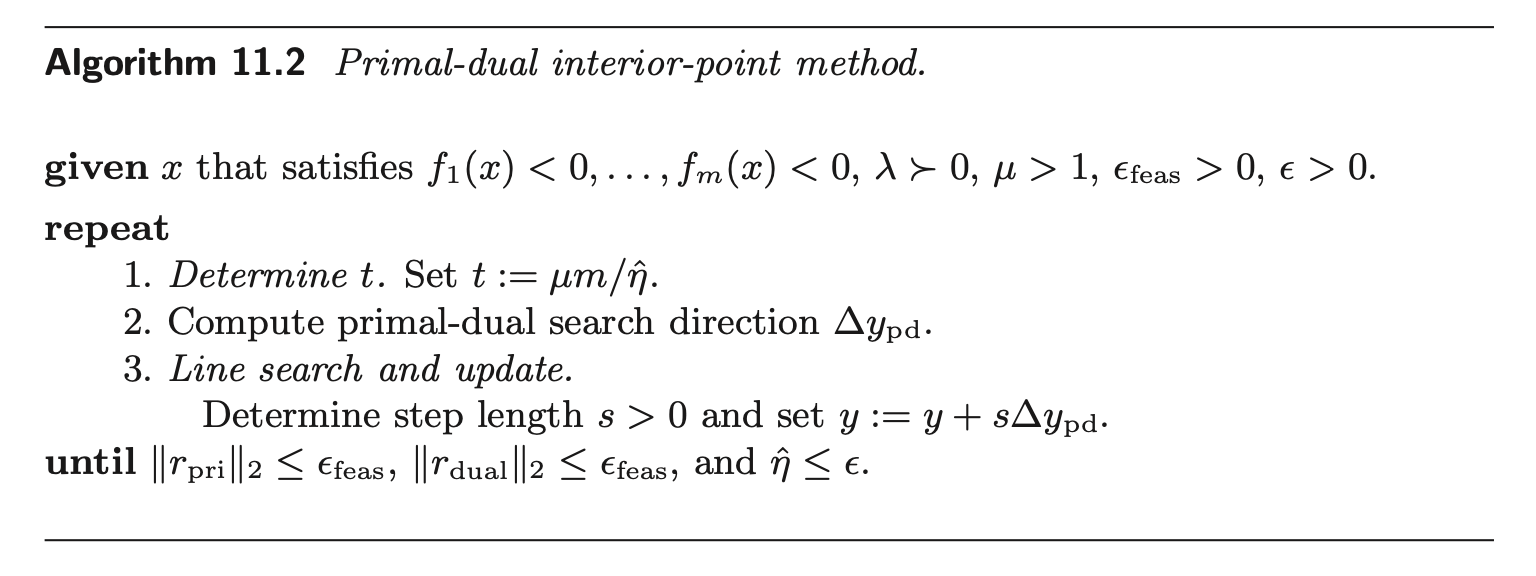
\includegraphics[width=0.7\textwidth]{PDIPOPT.png} 
\end{figure}

Adapt it to our problem, the computation details is as follows: Denote
\begin{equation}
    f(x) = (f_1(x),\dots,f_m(x))^T\text{ and }Df(x)^T = (\nabla f_1(x),\dots,\nabla f_m(x)).
\end{equation}
Define
\begin{equation}
    r_t(x,\lambda) = \begin{pmatrix}
    \nabla f_0(x)+Df(x)^T\lambda\\
    -diag(\lambda)f(x)-\frac{1}{t}\boldsymbol{1}
    \end{pmatrix}=:\begin{pmatrix}
        r_{\text{dual}}\\
        r_{\text{cent}}
    \end{pmatrix}.
\end{equation}
The system we need to solve is
\begin{equation}
    r_t(y+\Delta y) \approx r_t(y)+D r_t(y) \Delta y=0 \Rightarrow \Delta y=-D r_t(y)^{-1} r_t(y).
\end{equation}
Plug in the definition of $r_t$, we have
\begin{equation}
    \left(\begin{array}{cc}
\nabla^2 f_0(x)+\sum_{i=1}^m \lambda_i \nabla^2 f_i(x) & D f(x)^{T} \\
-\operatorname{diag}(\lambda) D f(x) & -\operatorname{diag}(f(x))
\end{array}\right)\left(\begin{array}{c}
\Delta x \\
\Delta \lambda
\end{array}\right)=-\left(\begin{array}{c}
r_{\text {dual }} \\
r_{\text {cent }}
\end{array}\right)
\end{equation}
From the second line, we can represent $\Delta \lambda$ with $\Delta x$:
\begin{equation}
    \Delta \lambda = -\operatorname{diag}(f(x))^{-1} \operatorname{diag}(x) D f(x) \Delta x+\operatorname{diag}(f(x))^{-1} r_{\text {cent }}.
\end{equation}
Plug it back into the first line, we have
\begin{equation}
    \left(\nabla^2 f_0(x)+\sum_{i=1}^m \lambda_i \nabla^2 f_i(x)+\sum_{i=1}^m \frac{\lambda_i}{-f_i(x)} \nabla f_i(x) \nabla f_i(x)^{\top}\right) \Delta x=-\left(\nabla f_0(x)+\frac{1}{t} \sum_{i=1}^m \frac{1}{-f_i(x)} \nabla f_i(x)\right).
\end{equation}
Now we consider our problem, we know the matrix
\begin{equation}
    \begin{aligned}
        &\nabla^2 f_0(x)+\sum_{i=1}^m \lambda_i \nabla^2 f_i(x)+\sum_{i=1}^m \frac{\lambda_i}{-f_i(x)} \nabla f_i(x) \nabla f_i(x)^{\top}\\
        &=\left(\begin{array}{ll}
M_{\perp}^{\top} M_{\perp}+\operatorname{diag}\left(-\frac{\xi}{l}-\frac{\eta}{u}\right) & \operatorname{diag}\left(-\frac{\xi}{l}+\frac{\eta}{u}\right) \\
\operatorname{diag}\left(-\frac{\xi}{l}+\frac{\eta}{u}\right) & \operatorname{diag}\left(-\frac{\xi}{l}-\frac{\eta}{u}\right)-\frac{\lambda}{g} 11^{\top}
\end{array}\right),
    \end{aligned}
\end{equation}
where $\xi$, $\eta$, and $\lambda$
 are the dual variables corresponding to $l, u, g$, respectively. The matrix used for preconditioner in CG is
 \begin{equation}
     \left(\begin{array}{ll}
I+\operatorname{diag}\left(-\frac{\xi}{l}-\frac{\eta}{u}\right) & \operatorname{diag}\left(-\frac{\xi}{l}+\frac{\eta}{u}\right) \\
\operatorname{diag}\left(-\frac{\xi}{l}+\frac{\eta}{u}\right) & \operatorname{diag}\left(-\frac{\xi}{l}-\frac{\eta}{u}\right)
\end{array}\right)
 \end{equation}
 Also, we have
 \begin{equation}
     -\left(\nabla f_0(x)+\frac{1}{t} \sum_{i=1}^m \frac{1}{-f_i(x)} \nabla f_i(x)\right)=\left(\begin{array}{c}
-M_{\perp}^{\top} M_{\perp} \beta+M_{\perp}^{\top} z+\frac{1}{t}\left(-\frac{1}{l}+\frac{1}{n}\right) \\
\frac{1}{t}\left(-\frac{1}{l}-\frac{1}{u}+\frac{1}{g} 1\right)
\end{array}\right).
 \end{equation}
 Thus, the search direction for dual variable is
 \begin{equation}
     -\left(\begin{array}{c}
\frac{\xi}{l(x)} \\
\frac{\eta}{\mu(x)} \\
\frac{\lambda}{g(x)}
\end{array}\right) \odot\left(\begin{array}{c}
-\Delta \beta-\Delta c \\
\Delta \beta-\Delta c \\
\boldsymbol{1}^{\top} \Delta c
\end{array}\right)-\left(\begin{array}{c}
\xi \\
\eta \\
\lambda \\
\end{array}\right)-\frac{1}{t}\left(\begin{array}{c}
\frac{1}{l} \\
\frac{1}{h} \\
\frac{1}{g}
\end{array}\right)
 \end{equation}

We perform a numerical experiment on a 1d example with $n=20$. The missing probability is 0.1. If $d$ is large enough such that the solution $\beta$ is not sparse, the algorithm performs well with the following 
\begin{figure}[H]
	\centering
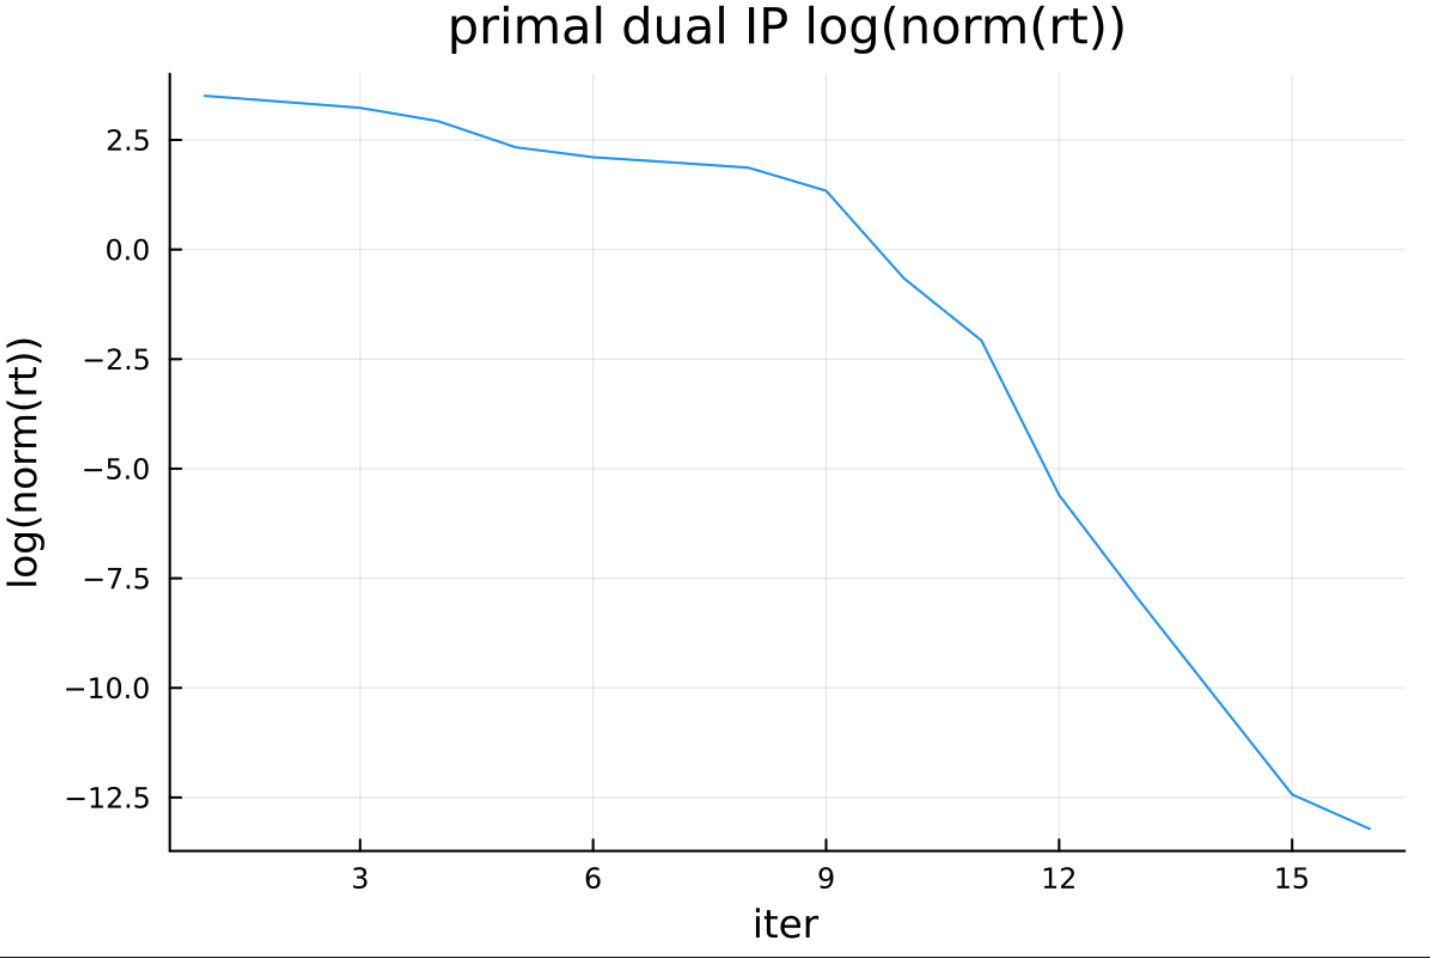
\includegraphics[width=0.6\textwidth]{Interior Point Method/subgradplot2_fig/PDrnorm.png} 		  \caption{primal-dual IP: log(norm(rt))}
\end{figure}
However, when $d$ is small to force a sparse solution, the algorithm is off when $r_t$ is small. When $r_t$ is small, the condition number of the matrix $\left(\nabla^2 f_0(x)+\sum_{i=1}^m \lambda_i \nabla^2 f_i(x)+\sum_{i=1}^m \frac{\lambda_i}{-f_i(x)} \nabla f_i(x) \nabla f_i(x)^{\top}\right)$ becomes large. Then with the search direction solved from the linear system, the line search step never ends.
%References
%\printbibliography
%\appendix



\end{document}
